\begin{figure}[h]
\centering
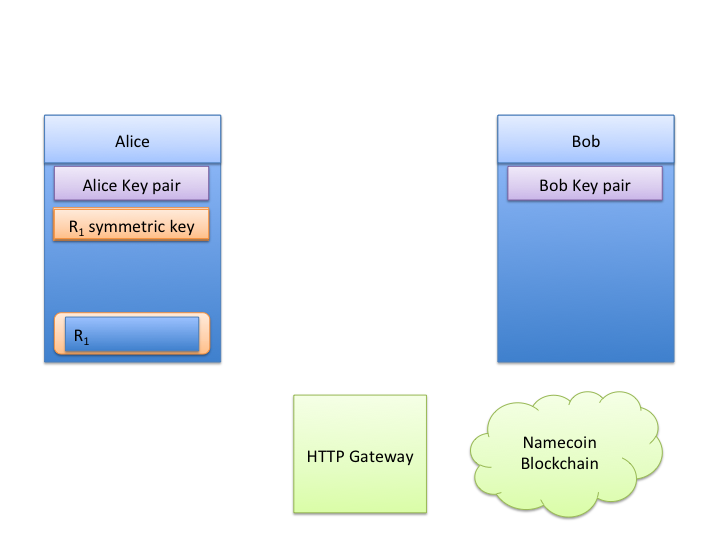
\includegraphics[width=\textwidth,height=0.2\paperheight,keepaspectratio
]{slides/Slide1.png}
\caption{Alice and Bob have added each other's identities as \emph{friends}. Alice has a resource $R_1$ that she wants to share with Bob. $R_1$ is encrypted with a symmetric secret key.}
\label{fig:slide1}
\end{figure}
\begin{figure}[h]
\centering
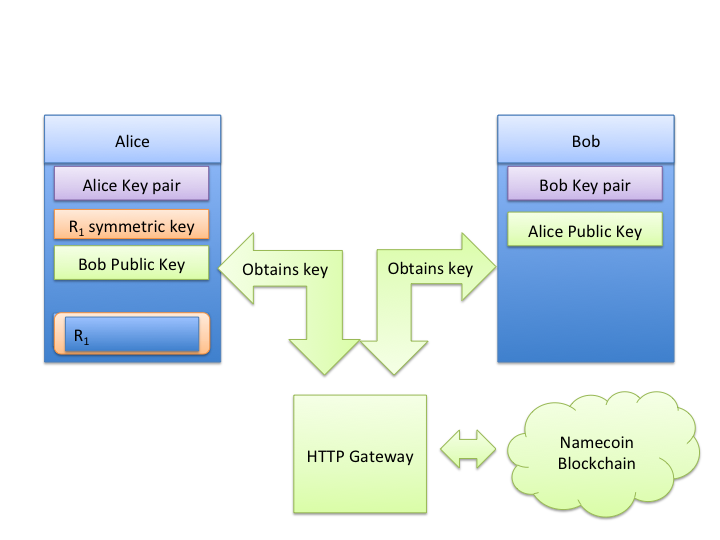
\includegraphics[width=\textwidth,height=0.2\paperheight,keepaspectratio
]{slides/Slide2.png}
\caption{Alice and Bob both independently contact an HTTP gateway to get each other's public keys from the DHT. If they do not want to trust a third party, they could set up their own gateway or even add the keys manually.}
\label{fig:slide2}
\end{figure}
\begin{figure}[h]
\centering
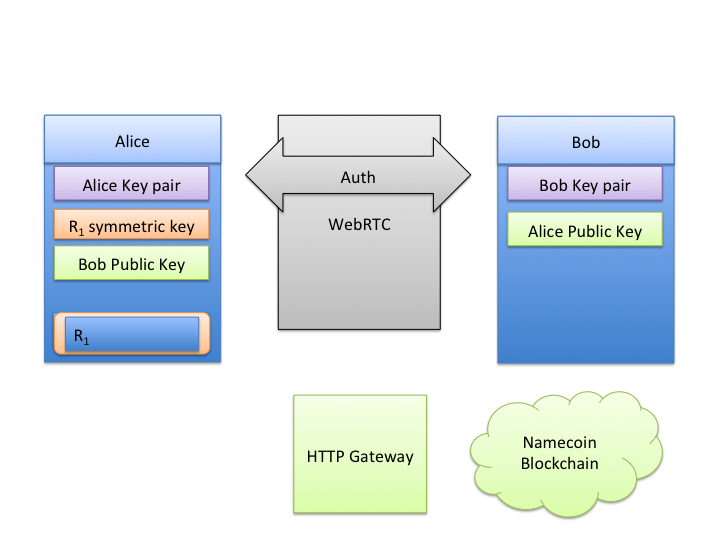
\includegraphics[width=\textwidth,height=0.2\paperheight,keepaspectratio
]{slides/Slide3.png}
\caption{Alice and Bob tells a central server that they want to communicate, for example by sending their friend lists. The server sets up a direct WebRTC connection between them. They use this channel to authenticate using standard public key cryptography.}
\label{fig:slide3}
\end{figure}
\begin{figure}[h]
\centering
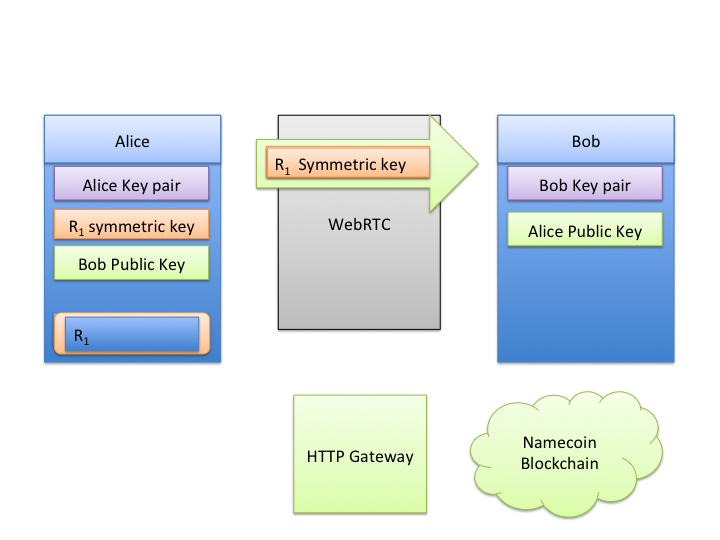
\includegraphics[width=\textwidth,height=0.2\paperheight,keepaspectratio
]{slides/Slide4.png}
\caption{Alice wants to share $R_1$, so she encrypts the key used to encrypt it with Bob's public key and sends it to Bob along with a reference ID that he can use to request it from Alice.}
\label{fig:slide4}
\end{figure}
\begin{figure}[h]
\centering
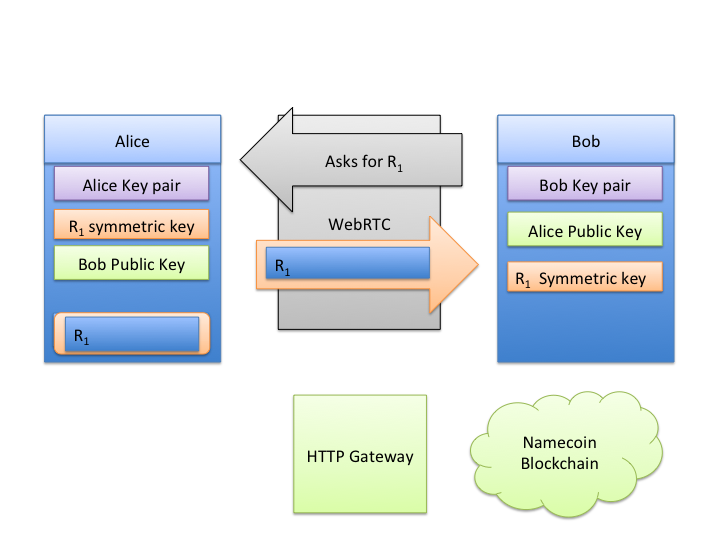
\includegraphics[width=\textwidth,height=0.2\paperheight,keepaspectratio
]{slides/Slide5.png}
\caption{Bob asks Alice for $R_1$. She responds by sending it, still encrypted with the key she just sent to Bob.}
\label{fig:slide5}
\end{figure}
\begin{figure}[h]
\centering
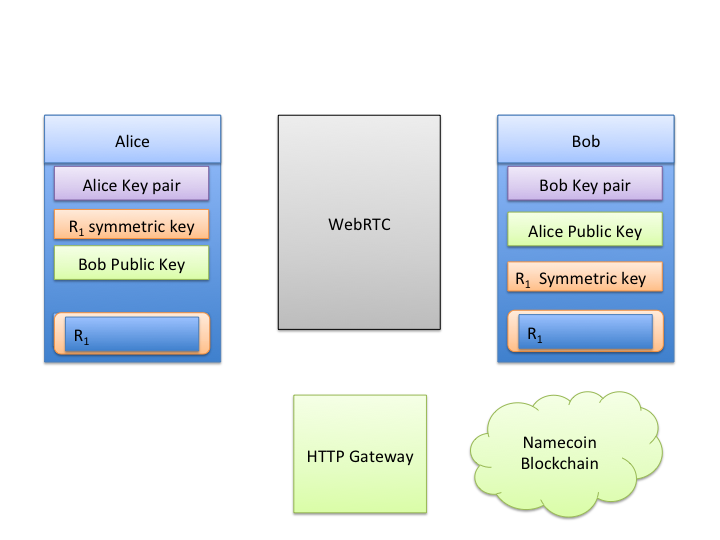
\includegraphics[width=\textwidth,height=0.2\paperheight,keepaspectratio
]{slides/Slide6.png}
\caption{The transaction is finished. Bob is now in possession of $R_1$ and the key used to encrypt it.}
\label{fig:slide6}
\end{figure}
